\section{Publish pipeline}
\paragraph{}
The publish pipeline (see figure below) is started by one of the following cvmfs\_server commands: either ingest, which extracts the content of a tarball into a repository, either publish, which creates a new repository snapshot by applying the changes made after the start of the transaction.
\begin{figure}[h]
\centering
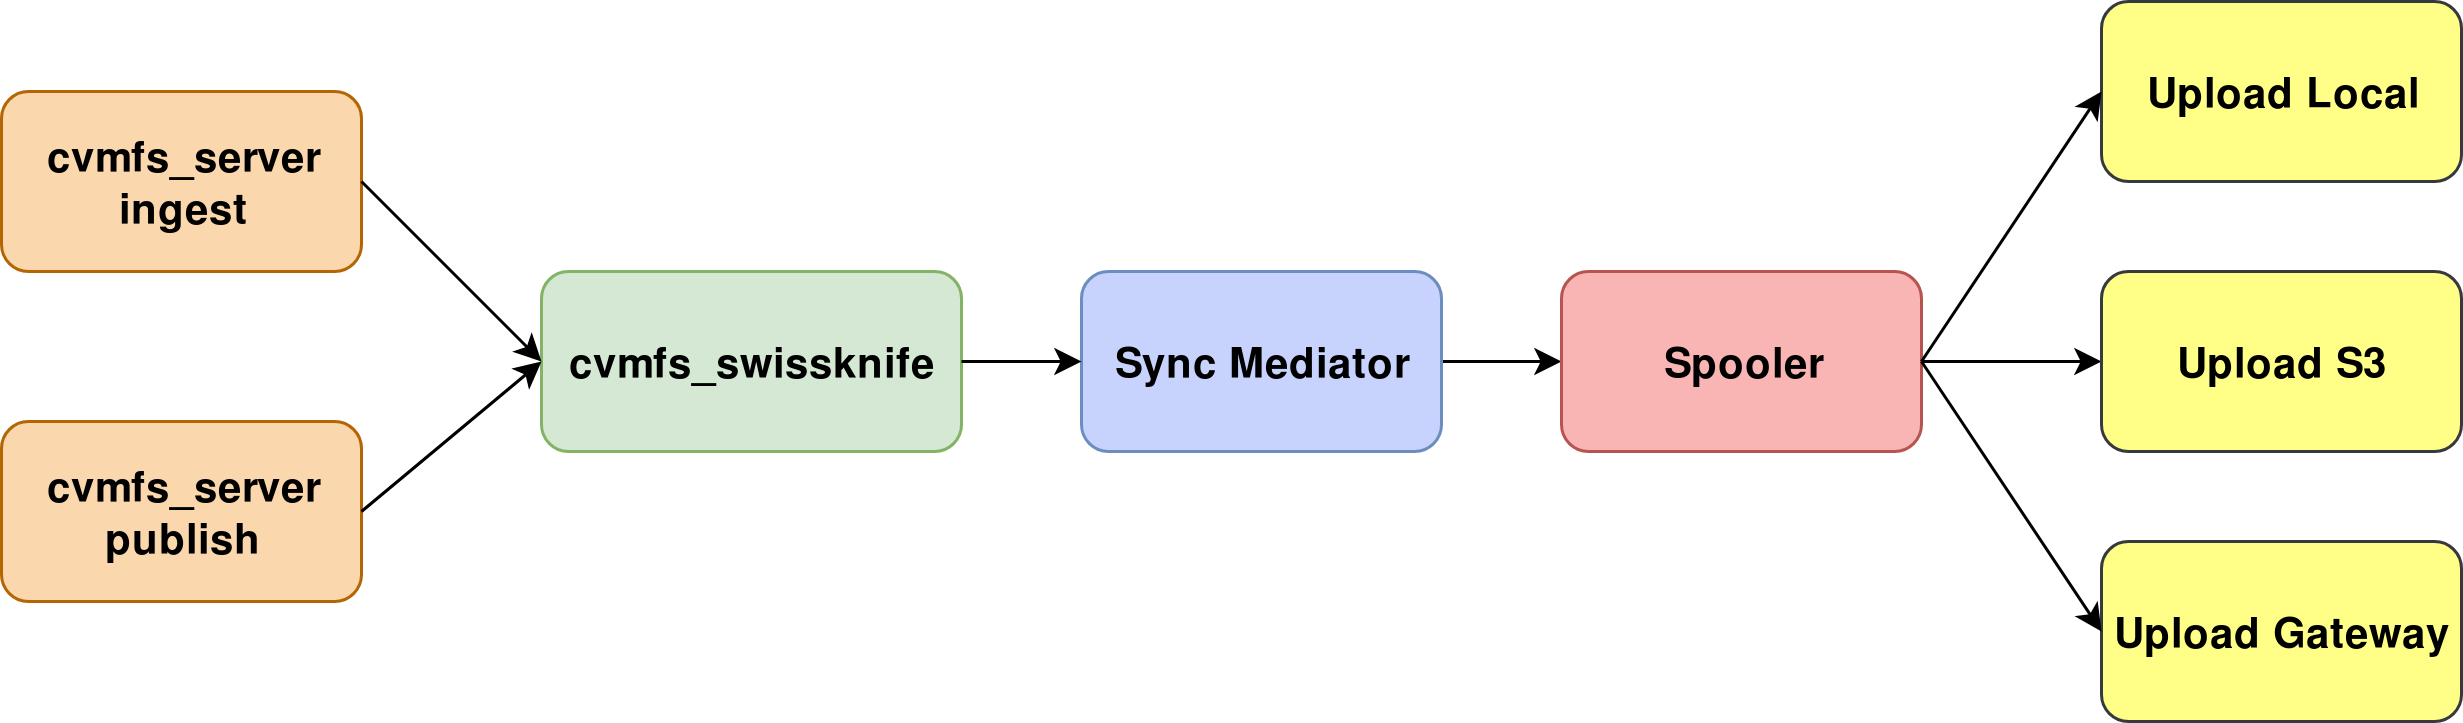
\includegraphics[scale=0.17]{figures/publish_pipeline2}
\caption{Publish pipeline}
\end{figure}
\par
The cvmfs\_swissknife binary identifies the command received and triggers the proper action for each command. In our case, the sync (publish) and ingest commands are shown. Both of these call the sync mediator element of the pipeline.
\par
The SyncMediator is an intermediate layer between the UnionSync implementation and the CatalogManager. Its main responsibility is to traverse newly created directories and to add all included files. Also, new and modified files are piped to the Spooler.
\par 
The SyncMediator is a good point to count the following metrics:
\begin{itemize}
  \item number of added/removed/changed files
  \item number of added/removed/changed directories
  \item number of added/removed bytes
\end{itemize}

\par
The Spooler is the entry point to the general file processing facility of the CVMFS backend. It works with a two-stage approach:
\begin{enumerate}
  \item Process file content
  \begin{itemize}
    \item create smaller file chunks for big input files
    \item compress the file content (optionally chunked)
    \item generate a content hash of the compression result
    \end{itemize}
  \item Upload the file (it supports different upload paths: local, S3, ...)
\end{enumerate}

\par 
\par
There are a number of different entities involved in the processing of a file content:
\begin{itemize}
\item Spooler            - general steering tasks ( + common interface )
\item IngestionPipeline  - chunking, compression and hashing of files
\item AbstractUploader   - abstract base class for uploading facilities
\item Concrete Uploaders - upload functionality for various backend storages
\end{itemize}

\par
At the AbstractUploader level and at the Concrete Uploaders I added my contribution for counting the compressed data size and the number of duplicated objects found.


\begin{figure}[h]
\centering
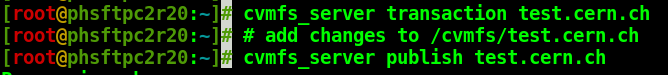
\includegraphics[scale=0.5]{figures/publish_terminal}
\caption{Publish workflow in a simple scenario}
\end{figure}

\section{Garbage collector}

\par The GarbageCollector is figuring out which data objects (represented by
their content hashes) can be deleted as outdated garbage.
Garbage collection is performed on the granularity of catalog revisions, thus
a complete repository revision is either considered to be outdated or active.
This way, a mountable repository revision stays completely usable (no nested
catalogs or data objects become unavailable). A revision is defined by its
root catalog; the revision numbers of nested catalogs are irrelevant, since
they might be referenced by newer (preserved) repository revisions.
This way, garbage objects are those that are \textbf{not} referenced by any of the preserved root catalogs or their direct subordinate nested catalog try.

It use a two-stage approach:
\begin{enumerate}
    \item \textbf{Initialization}:  The GarbageCollector is reading all the catalogs that are meant to be preserved. It builds up a filter containing all content hashes that will \textbf{not} be deleted
    \item \textbf{Sweeping}: The initialized filter is presented with all content hashes found in condemned catalogs and decides if they are referenced by the preserved catalog revisions or not.
\end{enumerate}

\begin{figure}[h]
\centering
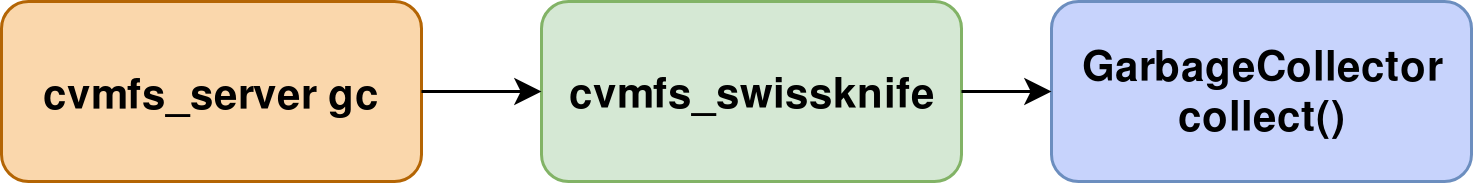
\includegraphics[scale=0.17]{figures/gc_pipeline}
\caption{Garbage collector pipeline}
\end{figure}
\paragraph{}
The Garbage collector pipeline follows a similar pattern (similar to the publish pipeline in the first two blocks): cvmfs\_server gc command uses cvmfs\_swissknife binary and then it calls the collect function from the GarbageCollector class which:
\begin{itemize}
    \item \textbf{Analyze the preserved CatalogTree}
    \item \textbf{Checks the Preserved Revisions}
    \item \textbf{Calls the Sweep function}
\end{itemize}

\paragraph{}In order to count number of preserved catalogs, number of condemned catalogs, number condemned objects and optionally the number of condemned bytes I changed the \textbf{Sweeping phase} by increment the thread safe counters. 
\paragraph{}I made optional the count of the condemned bytes because this might increase the garbage collector runtime. This measurement uses the stat system call many times which means many context switches that leads to some overhead, but further test should be run in order to evaluate the actual impact.
\paragraph{} In order to activate this optional measurement \textbf{CVMFS\_EXTENDED\_GC\_STATS} variable needs to be set in the server.conf file.
\begin{figure}[h]
\centering
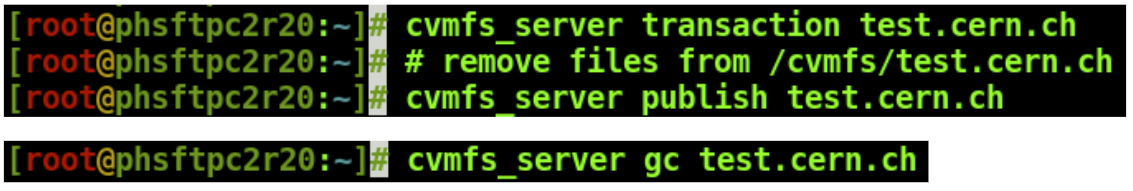
\includegraphics[scale=0.5]{figures/gc_workflow}
\caption{Garbage collector usage in a simple scenario}
\end{figure}

\par
All the statistics are stored locally in a SQLite file.
\par
In order to change the location of the SQLite file \textbf{CVMFS\_STATISTICS\_DB} variable needs to be changed. The default location is ``/var/spool/cvmfs/REPO\_NAME/stats.db`` .